\section{Vista Lógica}

\subsection{Entidades del dominio del negocio}

\textbf{Consulta (Query)}: Representa una operación a realizar sobre un conjunto determinado de datos. Cada operación es específica y se aplica a un conjunto de datos particular.

\textbf{Menu Item, Store, Transaction Item, Transaction}: Entidades sobre las que se aplican las consultas.

\subsection{Entidades del dominio del sistema}

\textbf{Plan de Ejecución (Execution Plan)}: Representa la secuencia de tareas que deben ejecutarse para resolver una consulta. Algunas tareas pueden ejecutarse en paralelo o en un orden específico según la optimización.

\textbf{Tarea (Task)}: Representa una transformación que un nodo debe realizar sobre uno o varios conjuntos de datos. Estas transformaciones pueden ser: Select, Project, Sort, Group by y Join. Cada tarea contiene la operación a ejecutar, la ubicación de los datos de origen y la ubicación de destino donde se almacenará el resultado.

\begin{figure}[H]
    \centering
    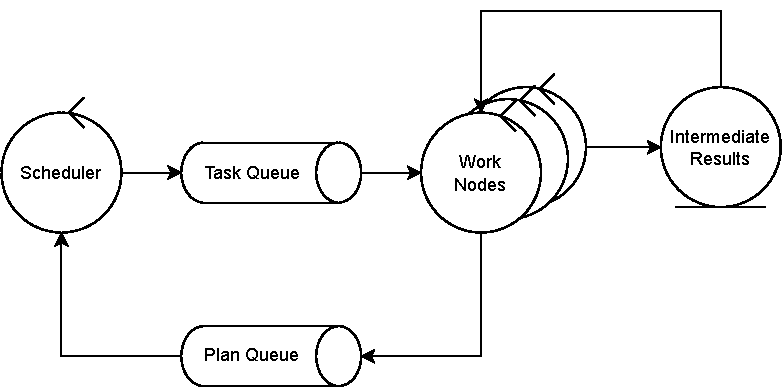
\includegraphics[width=1\textwidth]{img/robustez_entidades_principales.pdf}
    \caption{Diagrama de robustez entre las entidades principales}
\end{figure}